% ---------------------------- Preamble starts here ----------------------------

\documentclass[aspectratio=169]{beamer} %Remove [aspectratio=169] to get non-wide 4:3 slide aspect ratio

%-----------------------------------------------
% --- Set beamer theme
\usetheme{Metropolis}
\setbeamertemplate{footline}{}				% Remove automatic footer
\setbeamertemplate{navigation symbols}{}	% Comment this line to display navigation symbols

%-----------------------------------------------
% Load i2i symbol
\addtobeamertemplate{frametitle}{}{%
\begin{textblock*}{\linewidth}(0cm,7.4cm) % Replace with (0cm, 8cm) if using non-wide slide aspect
	
\includegraphics[width=\linewidth]{../../Common-Resources/img/Footer.png}
\end{textblock*}}

%-----------------------------------------------
% --- Load packages
\usepackage{textpos}		% To align objects correctly
\usepackage{multicol}		% To right in multiple columns
\usepackage{color}			% To color text

%-----------------------------------------------
% --- Include link to last commit
\usepackage{xstring}
\usepackage{catchfile}

%Set this user input
\newcommand{\gitfolder}{../../../.git} %relative path to .git folder from .tex doc
\newcommand{\reponame}{worldbank/dime-github-trainings} % Name of account and repo be set in URL

%Based on this https://tex.stackexchange.com/questions/455396/how-to-include-the-current-git-commit-id-and-branch-in-my-document
\CatchFileDef{\headfull}{\gitfolder/HEAD.}{} 				%Get path to head file for checked out branch
\StrGobbleRight{\headfull}{1}[\head]						%Remove end of line character
\StrBehind[2]{\head}{/}[\branch]							%Parse out the path only
\CatchFileDef{\commit}{\gitfolder/refs/heads/\branch.}{}	%Get the content of the branch head
\StrGobbleRight{\commit}{1}[\commithash]					%Remove end of line characted

%Build the URL to this commit based on the information we now have
\newcommand{\commiturl}{\url{https://github.com/\reponame/commit/\commithash}}

%-----------------------------------------------
% --- Add your information here
\title{An intro to Git and GitHub - Team Maintainer}
\author{DIME Analytics}
\institute{DIME - The World Bank - \trainingURL{https://www.worldbank.org/en/research/dime}}
\date{\today}

\newcommand{\trainingURL}[1]{{\color{blue}\url{#1}}}

\newcommand{\traininerUsername}{kbjarkefur}
\newcommand{\repoName}{\traininerUsername/lyrics-Jun17}
\newcommand{\trainingRepoURL}[1]{\trainingURL{github.com/\repoName #1}}
\newcommand{\trainerEmail}{\trainingURL{kbjarkefur@worldbank.org} }


% ---------------------------- Preamble ends here ----------------------------

\begin{document}

\begin{frame}

\includegraphics[width=\textwidth]{../../Common-Resources/img/Header.png}
\vspace{-0.2cm}
\titlepage 	 % Opening slide, prints inform
\end{frame}

\begin{frame}
\frametitle{Objectives}

This is the topics that we will cover in this training:
	\begin{itemize}
		\item Why do we bother with teams?
		\item Quick guide to how to do team maintainer tasks
		\item What other tasks do we ask the team maintainers to help us with?
	\end{itemize}
\end{frame}


%%%%%%%%%%%%%%%%%%%%%%%%%%%%%%%%%%%%%%%%%%%%%%%%%%%%%%%%%
%% Why bither with teams?

\begin{frame}
	\frametitle{Objectives}
	
	\begin{itemize}
		\item As default we do not give the project teams admin access to the repos
		
		\item With admin access you can do potentially destructive actions -- such as deleting the whole repo and all its history. 
		
		\item We still want you to give access to the teams to add and remove users from the repo without having to ask DIME Analytics each time.
		
		\item On GitHub, Teams can be used to control access to repos without giving admin access

	\end{itemize}
\end{frame}

\begin{frame}
	\frametitle{GitHub Teams Work Flow}

	\begin{columns}[c]
		
		\column{.60\textwidth} % Left column and width
		\begin{itemize}
			\item DIME Analytics creates a team
			\item DIME Analytics makes one team member the \textit{team maintainer}
			\item DIME Analytics creates a repo and adds the team to the repository
			\item The team maintainer add and remove user to the team to grant and revoke access to the repo
			\item Only users added to the DIME organization account can be added to teams
		\end{itemize}
		
		\column{.40\textwidth} % Right column and width
		\begin{figure}
			\centering
			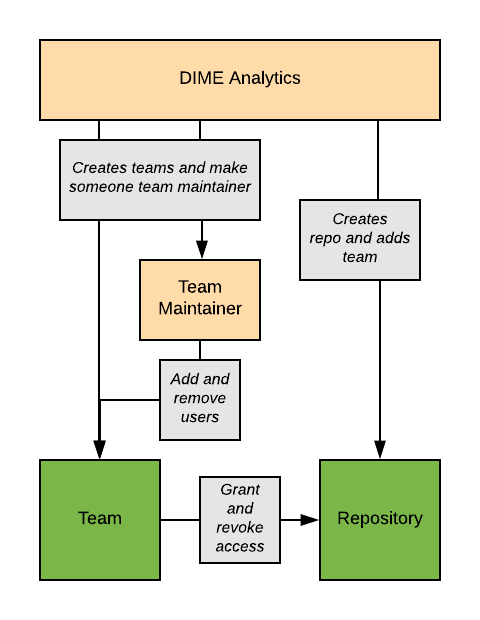
\includegraphics[width=1\linewidth]{./img/teams-workflow}
			\label{fig:finaldoccartoon}
		\end{figure}
		
	\end{columns}
\end{frame}


\begin{frame}{Useful links}
	\begin{itemize}
	  \item All DIME Analytics GitHub resources: \trainingURL{https://github.com/worldbank/dime-github-trainings}. For example:
		\begin{itemize}
			\item DIME Analytics GitHub Templates (for example .gitignore): \trainingURL{https://github.com/worldbank/dime-github-trainings/tree/master/GitHub-resources/DIME-GitHub-Templates}
			\item DIME Analytics GitHub Roles: \trainingURL{https://github.com/worldbank/dime-github-trainings/blob/master/GitHub-resources/DIME-GitHub-Roles/DIME-GitHub-roles.md}
		\end{itemize}
		\item Markdown cheat sheet (how to format text on GitHub.com):  \trainingURL{https://www.markdownguide.org/cheat-sheet/}
		\item DIME GitHub Account admin info and instructions: \trainingURL{https://github.com/dime-worldbank/dime-account-admin}
	\end{itemize}
\end{frame}


\begin{frame}{Version control}
	At the point of compiling this Beamer presentation, the most recent commit was:

	\commiturl

\end{frame}



\end{document}
